%!TEX root=finmath1.tex
\chapter{Модель Блэка--Шоулза}
\label{ch:bs}
\chaptertoc

Оставшаяся часть курса будет посвящена модели \bs\ (ее также называют моделью \bs"--~Мертона%
\footnote{Основные результаты были опубликованы Блэком и Шоулзом в работе \cite{BlackScholes73} в 1973 г., хотя получили и презентовали они их еще за несколько лет до этого.
Также в 1973 г.\ вышла статья Мертона \cite{Merton73}, содержащая более общие результаты и более математически строгая.})
и ее вариантам.
В этой лекции мы опишем модель в самом базовом виде и получим формулу \bs\ для цен европейских опционов колл и пут.

Мы будем следовать мартингальному подходу, который более удобен, чем оригинальный вывод, основанный на дифференциальных уравнениях (об этом методе будет немного сказано в последней части лекции).


\section{Описание модели}

\subsection{Активы и торговые стратегии}

Будем считать заданным вероятностное пространство $(\Omega, \F, \FF, \P)$, на котором определено стандартное броуновское движение $W=(W_t)_{t\in[0,T]}$.
Горизонт времени $T$ конечен.
Фильтрация $\FF=(\F_t)_{t\in[0,T]}$ порождена броуновским движением и пополнена (и, следовательно, непрерывна справа; см.\ сноску на стр.~\pageref{8:f:brownian-filtration}), причем $\F=\F_T$.

В модели имеются два актива, рисковый (акция) и безрисковый (денежный счет).
Цена безрискового актива $B=(B_t)_{t\in[0,T]}$ задается формулой
\[
B_t = B_0 e^{rt},
\]
\te\ представляет собой инвестирование в денежный рынок с постоянной процентной ставкой $r$, начисляемой непрерывным образом%
\footnote{Пусть за промежуток времени $[0,t]$ проценты начисляются $n$ раз, т.е.\ сумма на счете каждый раз увеличивается в $1+rt/n$ раз.
Тогда единица валюты, вложенная в такой актив в момент времени $0$, превратится в $(1+rt/n)^n$ единиц в момент $t$.
Переходя к пределу $n\to\infty$ (непрерывное начисление процентов) получаем $e^{rt}$.}.
Далее без ограничения общности считаем, что $B_0=1$.
Часто будет также удобно использовать дифференциальное представление для $B_t$:
\[
d B_t = r B_t dt, \qquad B_0=1.
\]

Цена рискового актива $S=(S_t)_{t\in[0,T]}$ задается геометрическим броуновским движением со сносом $\mu$ и волатильностью $\sigma>0$:
\[
S_t = s_0 e^{\sigma W_t + (\mu-\sigma^2/2)t}, \qquad s_0 > 0,
\]
или, в дифференциальной форме,
\[
d S_t = \mu S_t dt + \sigma S_t d W_t, \qquad S_0=s_0.
\]

\begin{definition}
\emph{Торговой стратегией} в модели Блэка--Шоулза называется пара измеримых согласованных процессов $\pi=(G,H)$, где процесс $G=(G_t)_{t\in[0,T]}$ выражает количество единиц безрискового актива в портфеле в момент времени $t$, а процесс $H=(H_t)_{t\in[0,T]}$ -- количество единиц рискового актива.
Пару значений $\pi_t=(G_t,H_t)$ будем называть \emph{портфелем} в момент времени $t$.

Считается, что процессы $G$ и $H$ должны удовлетворять условиям
\begin{equation}
\label{9:pi-integrals}
\int_0^T |G_t| dt < \infty, \qquad \int_0^T |H_t|^2 dt < \infty,
\end{equation}
\te\ $G\in\PP^1_T$ и $H\in\PP^2_T$.
\end{definition}

\begin{definition}
\emph{Стоимостью портфеля} стратегии $\pi$ называется процесс 
\[
V_t^\pi = G_t B_t + H_t S_t.
\]
Стратегия называется \emph{самофинансируемой}, если 
\begin{equation}
\label{9:sf}
d V_t^\pi = G_t d B_t + H_t d S_t.
\end{equation}
\end{definition}

Определение портфеля как пары $(G,H)$ и определение стоимости $V_t^\pi$ аналогичны моделям с дискретным временем.
Условие самофинансируемости \eqref{9:sf} получается формальным переходом к пределу в дискретной модели.
Действительно, его можно понимать как непрерывный аналог соотношения
\label{9:self-financing-discrete}
\[
\Delta V_t^\pi = G_t\Delta B_t + H_t \Delta S_t,
\]
где $\Delta$ обозначает изменение величины за <<бесконечно малый>> промежуток времени.
Это в точности условие самофинансируемости в дискретном времени (см.~предложение~\ref{gen:p:sf} в лекции \ref{ch:general}). 
Уравнение \eqref{9:sf} нужно, как обычно, понимать в интегральном смысле, \te
\[
\begin{split}
V_t^\pi &= V_0^\pi + \int_0^t G_u d B_u + \int_0^t H_u d S_u \\
&= V_0^\pi + \int_0^t (r G_u B_u + \mu H_u S_u) du + \int_0^t \sigma H_u S_u d W_u.
\end{split}
\]
Отсюда видно, что условие \eqref{9:pi-integrals} необходимо для того, чтобы интегралы были корректно определены.
В самом деле, из непрерывности процессов $B$, $G$ и условия \eqref{9:pi-integrals} следует, что $(rGB+\mu HS) \in \PP^1_T$ и $\sigma HS \in \PP^2_T$.

\begin{definition}
\emph{Дисконтированной ценой} рискового актива называется процесс 
$\tilde S_t = {S_t}/{B_t} = e^{-rt} S_t$. 
\emph{Дисконтированной стоимостью портфеля} стратегии $\pi$ называется процесс
$\tilde V_t^\pi = {V_t^\pi}/{B_t} = G_t + H_t \tilde S_t$.
\end{definition}

\begin{proposition}
Стратегия $\pi$ является самофинансируемой тогда и только тогда, когда
\begin{equation}
\label{9:sf-discounted}
d \tilde V_t^\pi = H_t d \tilde S_t.
\end{equation}
\end{proposition}

\begin{proof}
Если $\pi$ является самофинансируемой, то по формуле Ито
\begin{multline*}
d \tilde V_t^\pi = d(e^{-rt} V_t^\pi) = e^{-rt}(-r V_t^\pi dt + dV_t^\pi) 
= e^{-rt} (-rV_t^\pi dt + G_tdB_t + H_t d S_t) \\
= e^{-rt} (-rV_t^\pi dt +r  G_t B_tdt + H_t d S_t)
= -re^{-rt} H_tS_t dt + e^{-rt} H_t dS_t.
\end{multline*}
Кроме того,
\[
H_t d\tilde S_t = H_td(e^{-rt}S_t) = -re^{-rt}H_tS_t dt + e^{-rt}H_t dS_t.
\]
Правые части последних двух равенств совпадают, значит совпадают и левые.

Обратно, если $\pi_t$ удовлетворяет уравнению \eqref{9:sf-discounted}, то по формуле Ито
\begin{multline*}
d V_t^\pi = d (e^{rt} \tilde V_t^\pi) 
= re^{rt}\tilde V_t^\pi dt + e^{rt}d\tilde V_t^\pi 
= r V_t^\pi dt + e^{rt}H_td\tilde S_t \\
= r(G_tB_t + H_tS_t)dt+ (\mu - r)H_tS_t dt + \sigma H_tS_tdW_t \\
= r G_t B_t dt + H_t dS_t = G_t dB_t + H_tdS_t,
\end{multline*}
что есть в точности условие самофинансируемости.
\end{proof}

\begin{remark}
Аналогично подобному результату в дискретном времени (cм.\ замечание \ref{gen:r:sf-construction} в лекции \ref{ch:general}), формула \eqref{9:sf-discounted} позволяет легко задавать самофинансируемые стратегии: нужно задать только процесс $H$ и стоимость начального портфеля $V_0^\pi$, а процесс $G$ будет определен автоматически по формуле
\[
G_t = \tilde V_t^\pi - H_t \tilde S_t = V_0^\pi + \int_0^t H_u d \tilde S_u - H_t\tilde S_t.
\]  
\end{remark}


\subsection{Эквивалентная мартингальная мера, допустимые стратегии, отсутствие арбитража}

\begin{theorem}
\label{9:t:emm}
В модели Блэка-Шоулза существует единственная вероятностная мера $\Q\sim\P$, называемая \emph{эквивалентной мартингальной мерой}, такая, что процесс дисконтированной цены $\tilde S$ является мартингалом относительно $\Q$.
\end{theorem}

\begin{proof}
Существование следует из теоремы Гирсанова.
Действительно, мы можем построить меру $\Q$ такую, что процесс $W_t^{\Q} = W_t + \nu t$ является броуновским движением относительно $\Q$.
Возьмем $\nu=(\mu-r)/\sigma$.
Тогда
\[
dS_t = \mu S_t dt + \sigma S_t dW_t = \mu S_t dt + \sigma S_t d(W_t^{\Q} - \nu t) = r S_t dt + \sigma dW_t^{\Q}.
\]
Таким образом, относительно $\Q$ цена акции является геометрическим броуновским движением со сносом $r$, т.е.\ $S_t = s e^{\sigma W_t^{\Q} + (r-\frac{\sigma^2}{2})t}$.
Тогда $\tilde S_t = e^{-rt}S_t = s e^{\sigma W_t^{\Q} -\frac{\sigma^2}{2}t}$ является геометрическим броуновским движением с нулевым сносом, и, значит, мартингалом.

Доказательство единственности выходит за рамки нашего курса.
Его можно найти в книге \cite{Shiryaev98}, гл.~VII, \S\,4a.
\end{proof}

Следующее определение нужно, чтобы избежать арбитража (в отличие от дискретного времени, существование ЭММ в модели с непрерывным временем не гарантирует безарбитражность без ограничений на класс используемых стратегий; см.~замечание \ref{9:r:admissible} ниже).

\begin{definition}
\label{9:d:admissible}
Будем называть стратегию $\pi=(G,H)$ \emph{допустимой}, если $HS \in \L_T^2(Q)$, \te\ $\E^{\Q} \int_0^T (H_tS_t)^2 dt < \infty$.
\end{definition} 

\begin{remark}
Условие $HS \in \L_T^2(Q)$ эквивалентно тому, что $H\tilde S \in \L_T^2(Q)$, так как второй процесс получается из первого умножением на функцию $e^{-rt}$.
\end{remark}

\begin{proposition}
\label{9:p:admissible}
Если $\pi$ "--- самофинансируемая стратегия, то $V_t^\pi$ является локальным мартингалом относительно $\Q$. Если $\pi$ к тому же и допустима, то $V_t^\pi$  является квадратично интегрируемым мартингалом относительно $\Q$.
\end{proposition}

\begin{proof}
Так как $d\tilde S_t = \sigma \tilde S_t dW_t^{\Q}$, то имеем $d\tilde V_t = H_t d\tilde S_t = \sigma H_t S_t dW_t^{\Q}$.
Процесс $\sigma H_t \tilde S_t$ принадлежит пространству $\PP^2_T$, поэтому интеграл Ито является локальным мартингалом.
Для допустимой стратегии имеем $\sigma H\tilde S \in \L^2_T(\Q)$, поэтому интеграл Ито является квадратично интегрируемым мартингалом.
\end{proof}

Далее под словом ``стратегия'' мы всегда будем понимать допустимую самофинансируемую стратегию, если не оговорено иного. 

\begin{remark}
Из доказательств теоремы~\ref{9:t:emm} и предложения \ref{9:p:admissible} получаем следующие полезные формулы для стохастических дифференциалов
\begin{align}
\label{9:S-dynamics}
&d S_t = rS_t dt + \sigma S_t d W_t^{\Q},& 
  &d \tilde S_t = \sigma \tilde S_t d W_t^{\Q},\\
\label{9:V-dynamics}
&d V_t^\pi = r V_t dt + \sigma H_t S_t d W_t^{\Q},&
  &d \tilde V_t^\pi = \sigma H_t \tilde S_t d W_t^{\Q}.
\end{align}
\end{remark}

\begin{proposition}[отсутствие арбитража]
В модели Блэка-Шоулза не существует допустимой самофинансируемой стратегии $\pi$ такой, что $V_0^\pi = 0$, $V_T^\pi \ge 0$ и $\P(V_T^\pi > 0) > 0$.
\end{proposition}

\begin{proof}
Предположим, что такая стратегия существует.
Тогда $0 = \tilde V_0^\pi = \E^{\Q} \tilde V_T^\pi > 0$,
где второе равенство выполнено в силу мартингальности. Получаем противоречие.
\end{proof}

\begin{remark}
В дискретном времени справедлива первая фундаментальная теорема финансовой математики: безарбитражность равносильна существованию эквивалентной мартингальной меры.
Что можно сказать о справедливости этой теоремы в непрерывном времени? 

В модели Блэка--Шоулза мы ее фактически уже доказали: явно построили ЭММ и показали, что арбитража нет.
Для общих моделей ситуация становится сложнее.
Чтобы было справедливо аналогичное утверждение, надо, во-первых, ввести более сильное понятие отсутствия арбитража (часто используют так называемое условие NFLVR "--- \emph{no free lunch with vanishing risk}) и вместо эквивалентных мартингальных мер говорить об эквивалентных \emph{локальных} мартингальных мерах, \te\ таких мерах $\Q\sim\P$, что $\tilde S_t$ является локальным мартингалом относительно $\Q$.
Тогда можно доказать (\emph{теорема Дельбана"--~Шахермайера}), что условие NFLVR равносильно существованию эквивалентной локальной мартингальной меры.
Это очень трудный результат. 
\end{remark}

\begin{remark}
\label{9:r:admissible}
Зачем нужно условие допустимости?

Без этого условия можно построить арбитражную возможность -- самофинансируемую стратегию $\pi$ такую, что $V_0^\pi = 0$, $V_T^\pi > 0$ п.н.\ (см.~пример ниже).

В литературе часто используется другое определение допустимости: требуют, чтобы стоимость портфеля была ограничена снизу, т.е.\ $V_t^\pi \ge c$ для всех $t\in[0,T]$ с некоторой константой $c$.
Это условие является более подходящим для общих моделей рынков, в том числе неполных, где структура ЭММ  не известна в явном виде.
Такое условие, в отличие от нашего, инвариантно при замене исходной меры $\P$ на эквивалентную. 
С другой стороны, оно приводит к необходимости более аккуратных рассуждений, так как процесс стоимости портфеля является лишь локальным мартингалом относительно ЭММ.
Например, можно построить допустимую самофинансируемую стратегию $\pi$ такую, что $V_0^\pi  = 1$, а $V_T^\pi = 0$, \te\ стратегия <<сжигает деньги>>.
Тогда две стратегии, реплицирующие одно и то же платежное обязательство, могут иметь разную начальную стоимость ($X=0$ можно реплицировать нулевой стратегий и стратегией, сжигающей деньги), и, следовательно, нужно модифицировать определение цены репликации.
Подробнее об этих нюансах можно прочитать в книге \cite{EberleinKallsen19}, глава 11, раздел 7.

Чтобы избежать этих сложностей, мы используем более простое определение допустимости, благо в модели Блэка-Шоулза ЭММ существует, единственна, и имеет явный вид.
\end{remark}

\begin{example}[$*$]
Если не требовать допустимости, то возникнет арбитраж.
Для примера рассмотрим модель Блэка--Шоулса с параметрами $\mu=r=0$, $\sigma=1$.
Определим процесс 
\[
\xi_t = \int_0^t \frac{1}{1-s} d W_s, \qquad t\in[0,1).
\]
Пусть $\tau = \inf\{t: \xi_t = 1\}$.
Можно показать, что процесс $\xi_t$ равен $W_{{t}/({1-t})}$ по распределению, откуда следует, что $\tau<1$ \as\ 
Рассмотрим самофинансируемую стратегию $\pi_t=(G_t,H_t)$ с $V_0^\pi = 0$ и  
\[
H_t = \frac{1}{(1-t)S_t} \I(t\le \tau).
\]
Тогда
\[
V_1^\pi = \int_0^1 H_t d S_t = X_\tau = 1.
\]
Таким образом, $\pi$ "--- арбитражная возможность.
\end{example}


\section{Платежные обязательства и их цены}

\begin{definition}
\emph{Платежное обязательство европейского типа} отождествляется с $\F_T$-измеримой случайной величиной $X$ такой, что $\E^{\Q} X^2 < \infty$.

Платежное обязательство называется \emph{реплицируемым}, если существует допустимая самофинансируемая стратегия $\pi$ такая, что $V_T^\pi = X$ \as
\end{definition}

\begin{remark}
Условие $\E^{\Q} X^2 <\infty$ нужно для того, чтобы иметь возможность говорить о репликации с помощью допустимых стратегий, так как условие допустимости требует квадратичной интегрируемости стоимости портфеля.
\end{remark}

\begin{theorem}[полнота модели Блэка--Шоулза]
В модели Блэка--Шоулза любое платежное обязательство (в смысле определения выше) реплицируемо, и для него существует единственная реплицирующая стратегия.
\end{theorem}

\begin{proof}
Из теоремы о мартингальном представлении следует, что найдется единственный процесс $H'$ такой, что для величины $\tilde X = e^{-rT} X$ справедливо представление
\[
\tilde X = \E^{\Q} \tilde X + \int_0^T H'_t d W_t^{\Q},
\]
причем $H'\in\L^2(Q)$. Возьмем самофинансируемую стратегию с процессом $H_t = H'_t/\sigma \tilde S_t$ и начальной стоимостью $V_0^\pi = \E^{\Q} \tilde X$. Тогда 
\[
\tilde V_T^\pi = V_0^\pi + \int_0^T H_t d\tilde S_t = \E^{\Q} \tilde X + \int_0^T H'_t d W_t^{\Q} = \tilde X.
\]
Отсюда следует, что $V^\pi = X$, т.е.\ $\pi$ реплицирует $X$.

Единственность реплицирующей стратегии следует из единственности в теореме о мартингальном представлении.
\end{proof}

\begin{definition}
\emph{Ценой репликации} платежного обязательства $X$ называется процесс стоимости портфеля реплицирующей стратегии: $V_t^X = V_t^\pi$.
\end{definition}

Из того, что дисконтированная стоимость портфеля является мартингалом относительно ЭММ, получаем следующее утверждение.

\begin{theorem}
Цена репликации платежного обязательства $X$ в модели Блэка--Шоулза равна
\begin{equation}
V_t^X = e^{-r(T-t)} \E^{\Q} (X \mid \F_t).
\end{equation}
\end{theorem}

\begin{proof}
Имеем
\[
\tilde V_t^\pi = \E^{\Q} (\tilde V_T^\pi \mid \F_t) = e^{-rT} \E^{\Q} (X \mid \F_t), 
\]  
и для завершения доказательства вспомним, что $\tilde V_t^\pi = e^{-rt} V_t^\pi$.
\end{proof}

\begin{remark}
Следует обратить внимание на то, что параметр модели $\mu$ не входит в формулу для цены и не играет роли в ценообразовании деривативов.
\end{remark}

\begin{corollary}
\label{9:c:path-independent}
Пусть платежное обязательство имеет вид $X=f(S_T)$, где функция $f$ такова, что $|f(s)| \le c(1+ s^m)$ с некоторыми константами $c,m$.
Тогда цена репликации может быть представлена в виде $V_t^X = V(t,S_t)$, где $V(t,s)$ -- неслучайная функция, задаваемая формулой
\begin{equation}
\label{9:markov-price-int}
V(t,s) = e^{-r(T-t)}  \int_\R f(se^{\sigma x \sqrt{T-t}  + (r-\frac{\sigma^2}{2})(T-t)}) \phi(x) dx,  
\end{equation}
где $\phi(x)$ -- стандартная нормальная плотность.
Компонента $H$ реплицируемой стратегии задается формулой\footnote{Производная $V'_s$ называется \emph{дельтой} опциона, см.~раздел~\ref{9:ss:greeks}.
Стратегия с такой компонентой называется \emph{дельта-хеджирующей}.}
\begin{equation}
\label{9:delta-hedge}
H_t = V'_s(t,S_t).
\end{equation}
\end{corollary}
\begin{proof}
Из марковского свойства геометрического броуновского движения следует, что $\E^{\Q}(f(S_T) \mid \F_t) = \E^{\Q}(f(S_T) \mid S_t)$.
Тогда доказываемое представление $V_t^X=V(t,S_t)$ будет верно, если взять функцию
\begin{equation}
\label{9:markov-price}
V(t,s) = e^{-r(T-t)} \E^{\Q}(f(S_T) \mid S_t = s).
\end{equation}

Далее представим $S_T = S_t e^{\sigma (W_T^{\Q} - W_t^{\Q}) + (r-\frac{\sigma^2}{2})(T-t)}$ и воспользуемся тем, что $W_T^{\Q} - W_t^{\Q}$ имеет нормальное распределение с дисперсией $T-t$ и не зависит от $S_t$. Тогда, если записать математическое ожидание в виде интеграла по плотности, то получим формулу \eqref{9:markov-price-int}. 

Докажем \eqref{9:delta-hedge}. Достаточно будет показать, что если взять самофинансируемую стратегию с заданной компонентой $H$ и начальной стоимостью портфеля $V_0^\pi = V(0,S_0)$, то стоимость ее портфеля будет равна $V(t,S_t)$.

Применяя формулу Фейнмана--Каца%
\footnote{Для обоснования применимости формулы Фейнмана"--~Каца можно воспользовавшись аргументами из замечания \ref{8:r:feynman-kac} в лекции \ref{ch:ito-processes}.
Некоторую трудность в проверке представляют условия о существовании непрерывных производных у функции $V$ и ее не более чем степенной рост, но это можно сделать, благодаря тому, что есть явное представление по формуле \eqref{9:markov-price-int}.} к представлению \eqref{9:markov-price}, получаем, что $V(t,s)$ удовлетворяет уравнению
\[
V'_t(t,s) + rsV'_s(t,s) + \frac{\sigma^2}{2} s^2 V''_{ss}(t,s) = rV(t,s).
\]
Используя далее формулу \eqref{9:V-dynamics} и формулу Ито, получаем
\begin{multline*}
d (V_t^\pi - V(t,S_t)) = rV_t^\pi dt + \sigma S_t  H_t  d W_t^{\Q} \\- \Bigl(V'_t(t,S_t)dt + r S_tV'_s(t,S_t) dt + \sigma  S_tV'_s(t,S_t) dW_t^{\Q} + \frac{\sigma^2}2  S_t^2V''_{ss}(t,S_t) dt \Bigr)\\
 = r(V_t^\pi  - V'_t(t,S_t)) dt.
\end{multline*}
Это обыкновенное дифференциальное уравнение на $V_t^\pi - V(t,S_t)$, которое имеет единственное решение $V_t^\pi - V(t,S_t) = ce^{rt}$.
Так как начальное условие $V_0^\pi - V(0,S_0) = 0$, то этот процесс равен нулю для всех $t$.
\end{proof}

Заметим, что по ходу доказательства мы получили следующее уравнение c частными производными для цены платежного обязательства $X = f(S_T)$, называемое \emph{уравнением \bs}.

\begin{corollary}[уравнение \bs]
В условиях предыдущего следствия, функция цены $V(t,s)$ удовлетворяет уравнению
\begin{equation}
\label{9:bs-pde}
\left\{
\begin{aligned}
&V'_t(t,s) + rsV'_s(t,s) + \frac{\sigma^2}{2} s^2 V''_{ss}(t,s) = rV(t,s),
  \qquad t\in[0,T), s>0,\\
&V(T,s) = f(s), \qquad s>0.
\end{aligned}
\right.
\end{equation}

\medskip
\end{corollary}


\section{Формула \bs}
\label{9:s:bs}
\subsection{Формула}
Для функций выплат европейских опционов колл и пут ($f_{\text{call}}(s) = (s-K)^+, f_{\text{put}}(s) = (K-s)^+$) из следствия \ref{9:c:path-independent} получается известная формулу \bs\ (нужно вычислить интегралы в формуле \eqref{9:markov-price-int}, что остается в качестве упражнения).

\begin{corollary}[формула \bs]
Для цен европейских опционов колл и пут в модели \bs\ справедливы формулы
\begin{equation}
\label{bs1:bs-formula}
\begin{aligned}
&\VC(t,s) = s \Phi(d_1) - K e^{-r(T-t)} \Phi(d_2), \\
&\VP(t,s) = K e^{-r(T-t)} \Phi(-d_2) - s \Phi(-d_1),
\end{aligned}
\end{equation}
где $\Phi(x)$ обозначает стандартную нормальную функцию распределения, и
\begin{align*}
&d_1 = \frac{\ln(s/K) + (r+\sigma^2/2)(T-t)}{\sigma\sqrt{T-t}}, \\
&d_2 = d_1 - \sigma\sqrt{T-t} = \frac{\ln(s/K) + (r-\sigma^2/2)(T-t)}{\sigma\sqrt{T-t}}.
\end{align*}
\end{corollary}

\begin{remark}
Параметр времени входит в формулу \bs\ в виде разности $T-t$, выражающей \emph{время до экспирации} опциона.
Часто бывает удобнее работать именно с временем до экспирации, чем с временем после начала торговли. 
Несложно видеть, что $\VC(t,T,s) = \VC(0,T-t,s)$, где $\VC(t,T,s)$ обозначает цену опциона в момент времени $t$, имеющего время исполнения $T$, т.е.\ можно перенести отсчет времени в текущий момент $t$.
Аналогично для опционов пут.
\end{remark}

Отметим также полезное равенство "--- \emph{паритет цен колл-пут}.
Его можно получить как прямо из формулы \bs, так и применив рассуждения с репликацией подобно тому, как мы это делали в дискретном времени.

\begin{corollary}[паритет цен колл-пут]
В модели \bs\ для европейских опционов колл и пут с одинаковыми страйками и временем экспирации справедливо равенство
\[
\VC(t,s) - \VP(t,s) = s - K e^{-r(T-t)}.
\]
\end{corollary}


\subsection{Качественный анализ}
Зафиксируем время экспирации $T$ и будем обозначать цены опционов колл и пут как $\VC(t,s,K)$ и $\VP(t,s,K)$, чтобы подчеркнуть их зависимость от текущего времени (или времени до экспирации), цены акции и страйка.
\begin{proposition}
Для функций $\VC(t,s, K)$ и $\VP(t,s, K)$ при $t<T$ справедливы следующие утверждения.
\begin{enumerate}
\item \VC\ возрастает по $s$, убывает по $K$; $\VP$ убывает по $s$, возрастает по $K$.
\item Обе функции выпуклы по $s$ и по $K$.
\item $\VC = o(1)$, $\VP= Ke^{-r(T-t)} - s + o(1)$ при $s\to 0$.
\item $\VC = s - Ke^{-rT} + o(1)$, $\VP = o(1)$ при $s\to+\infty$.
\item $\VC = s + o(1)$, $\VP = o(1)$ при $K\to 0 $.
\item $\VC = o(1)$, $\VP = Ke^{-r(T-t)} - s + o(1)$ при $K\to+\infty$.
\item $\VC \to (s-K)^+$, $\VP \to (K-s)^+$ при $t\to T$.
\end{enumerate}
\end{proposition}

\begin{proof}
Первое свойство следует из вычисления производных цен опционов (нужно продифференцировать формулу \bs\ и убедиться, что, скажем, $\partial \VC/\partial s>0$; аналогично для других производных), второе "--- из вычисления вторых производных.

В третьем свойстве нужно воспользоваться тем, что $d_1,d_2 \to -\infty$ при $s\to0$. 
Следовательно, $\Phi(d_1),\Phi(d_2) \to 0$ и $\Phi(-d_1) = 1 - o(1)$, $\Phi(-d_2) = 1 - o(1)$.

В четвертом свойстве воспользуемся тем, что $d_1,d_2 \to +\infty$ при $s\to+\infty$ и применим аналогичные рассуждения (для вычисления асимптотики $s\Phi(d_2)$ представим $s\Phi(d_2) = s + s(\Phi(d_2)-1)$, и тогда из применения правила Лопиталя ко второму слагаемому следует, что оно есть $o(1)$).

Пятое и шестое свойства доказываются аналогично. Седьмое тоже получается несложным переходом к пределу.
\end{proof}

Используя это предложение, можно качественно изобразить цены опционов в зависимости от параметров, см.~рис.~\ref{9:f:bs}.
Два верхних графика изображают зависимость цены опционов от цены базового актива $s$ при фиксированном страйке $K=100$ и четырех различных значениях параметра времени до экспирации.
На двух нижних графиках показана зависимость цены опционов от страйка $K$ при фиксированной цене базового актива $s=100$.
На всех графиках процентная ставка равна $r=0.05$, волатильность $\sigma=0.2$.

\begin{figure}[h]
\centering
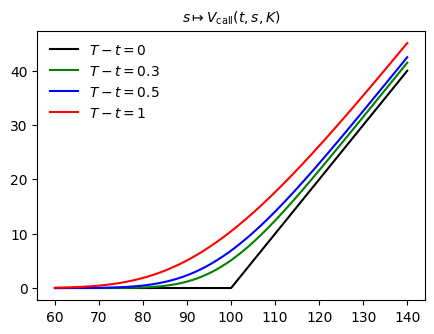
\includegraphics[height=5.2cm]{pic/callprice-s.png}\qquad
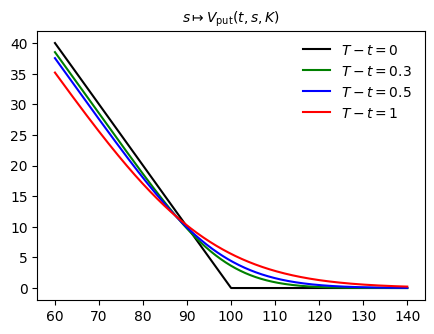
\includegraphics[height=5.2cm]{pic/putprice-s.png}\\
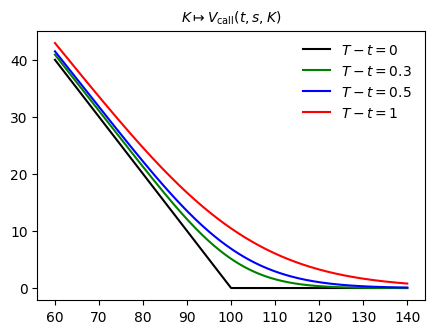
\includegraphics[height=5.2cm]{pic/callprice-k.png}\qquad
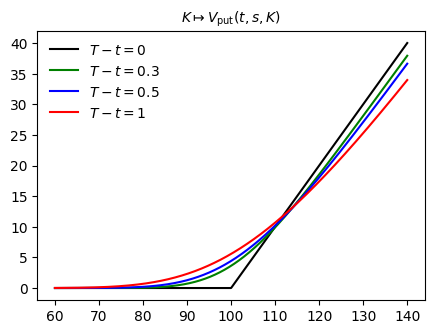
\includegraphics[height=5.2cm]{pic/putprice-k.png}
\caption{Цены опционов колл и пут в модели \bs.}
\label{9:f:bs}
\end{figure}


\subsection{Греки}
\label{9:ss:greeks}

\emph{Греками} (греческими буквами, Greeks) называются производные функции цены опциона по параметрам.

В модели \bs\ цены опционов колл и пут зависят от 5 параметров: цена базового актива $s$, время до экспирации $\tau:=T-t$, страйк $K$, процентная ставка $r$ и волатильность $\sigma$.
Страйк опциона не меняется, поэтому будем рассматривать цены как функции $\VC(s,\tau,r,\sigma)$ и $\VP(s,\tau,r,\sigma)$. 

Выделим следующие часто используемые греки:
\begin{align*}
\text{дельта}\ \Delta &= \frac{\partial V}{\partial s},&
  \text{гамма}\ \Gamma &= \frac{\partial^2 V}{\partial s^2},\\[0.5em]
\text{тета}\ \Theta &= \frac{\partial V}{\partial t} = - \frac{\partial V}{\partial \tau},&
  \text{ро}\ \rho &= \frac{\partial V}{\partial r},\\[0.5em]
\text{вега\footnotemark}\ \mathcal{V} &= \frac{\partial V}{\partial \sigma}.& &
\end{align*}
\footnotetext{Вега "--- это не греческая буква.}

В модели \bs\ греки можно вычислить аналитически.
Формулы приведены в таблице \ref{bs1:t:greeks}, сами вычисления остаются в качестве упражнения.

\begin{table}[h]
\centering
\renewcommand{\arraystretch}{1.25}
\begin{tabular}{|l|c|c|}
\hline
       & Колл & Пут \\\hline
$\Delta$ & $\Phi(d_1)$  & $\Phi(d_1) - 1$ \\\hline
$\Gamma$  & \multicolumn{2}{c|}{$\vphantom{\Bigg|} \dfrac{\phi(d_1)}{s\sigma\sqrt{\tau}}$} \\\hline
$\Theta$   & $\vphantom{\Bigg|} -\dfrac{s\phi(d_1)\sigma}{2\sqrt{\tau}} - rK e^{-r\tau} \Phi(d_2)$ &   $-\dfrac{s\phi(d_1)\sigma}{2\sqrt{\tau}} + rK e^{-r\tau} \Phi(-d_2)$ \\\hline
$\mathcal{V}$   & \multicolumn{2}{c|}{$s\phi(d_1)\sqrt{\tau}$} \\\hline
$\rho$     & $K\tau e^{-r\tau} \Phi(d_2)$  & $-K\tau e^{-r\tau} \Phi(-d_2)$ \\\hline
\end{tabular}
\caption{Греки опционов колл и пут в модели \bs.}
\label{bs1:t:greeks}
\end{table}

С помощью греков можно оценить изменение цены опциона при малом изменении параметров. Действительно, формально раскладывая по формуле Тейлора, получаем
\begin{multline*}
V(s+d s, \tau - d \tau, r+ dr, \sigma+ d\sigma)
\\= V(s,\tau,r,\sigma) + \Delta d s + \Theta d \tau + \mathcal{V} d \sigma + \rho d r + \frac12 \Gamma (d s)^2 + \ldots,
\end{multline*}
где $d$ обозначает малое приращение параметра. (Перед $d\tau$ для удобства стоит знак минус, так как время до экспирации уменьшается с течением календарного времени.)

Для понимания качественного поведения цены при изменении параметров полезно помнить знаки греков (см.~таблицу~\ref{9:t:greeks}).
Например, положительность дельты опциона колл означает, что его цена возрастает при росте цены базового актива; положительность веги обоих опционов означает, что их цена возрастает при увеличении волатильности и \td

\begin{table}[h]
\centering
\renewcommand{\arraystretch}{1.25}
\begin{tabular}{|l|c|c|}
\hline
       & Колл & Пут \\\hline
$\Delta$ & $+$  & $-$ \\\hline
$\Gamma$  & $+$  & $+$ \\\hline
$\Theta$   & $-$\makebox[0pt]{\phantom{$*$}$^*$} & $-$\makebox[0pt]{\phantom{$**$}$^{**}$} \\\hline
$\mathcal{V}$   & $+$  & $+$ \\\hline
$\rho$     & $+$  & $-$ \\\hline
\end{tabular}

\medskip
\parbox{0.78\textwidth}{\footnotesize
* За исключением некоторых опционов в деньгах ($s>K$), когда $r<0$.\\
** За исключением некоторых опционов в деньгах ($s<K$), когда $r>0$.
}

\caption{Знаки греков для опционов колл и пут.}
\label{9:t:greeks}
\end{table}

% \subsection{Другие термины, связанные с опционами}
% \begin{definition}
% Говорят, что опцион колл (или опцион пут) находтс 
% \end{definition}
% \begin{definition}
% Внутренней стоимостью опциона колл (или опциона пут) в момент $t$ называется величина $(S_t-K)^+$ (соответственно, $(K-S_t)^+$).

% Временной стоимостью опциона колл (или опциона пут) в момент $t$ называется величина $\VC_t - (S_t-K)^+$ (соответственно, $(K-S_t)^+$).
% \end{definition}


\section{\difficult\ Другой вывод уравнения Блэка--Шоулза}
Покажем, как можно было бы получить уравнение и формулу \bs\ без привлечения мартингалов, а используя только операции с дифференциалами "--- именно так рассуждали Блэк, Шоулз и Мертон в своих работах.
Будем работать с исходной вероятностной мерой $\P$ и броуновским движением $W$.

Рассмотрим платежное обязательство $X = f(S_T)$.
Ввиду марковости модели разумно предположить, что его цена выражается как функция $V(t,S_t)$. Тогда по формуле Ито имеем
\[
d V(t,S_t) = \Bigl(V'_t(t,S_t) + \mu S_t V'_s(t,S_t) + \frac{\sigma^2}2 S_t^2 V''_{ss}(t,S_t) \Bigr) dt + \sigma S_t V'_s(t,S_t) dW_t.
\]
Подберем теперь самофинансируемую стратегию $\pi=(G,H)$ с таким же стохастическим дифференциалом (и тогда она будет реплицировать платежное обязательство).
Из условия самофинансирования имеем
\[
d V_t^\pi = G_t d B_t + H_t d S_t = rG_t B_t dt + \mu S_t H_t dt + \sigma S_t H_t dW_t. 
\]
Приравнивая коэффициенты при $dt$ и $dW_t$ в этих двух выражениях, получаем
\begin{align*}
&(\text{при}\ dW_t)& &H_t = V'_s(t,S_t),\\
&(\text{при}\ dt)& &r B_t G_t + \mu S_t H_t = V'_t(t,S_t) + \mu S_t V'_s(t,S_t) 
  + \frac{\sigma^2 S_t^2}{2} V''_{ss}(t, S_t).
\end{align*}
Подставляя во второе уравнение $H_t = V'_s(t,S_t)$ и $G_t = V(t,S_t) - H_t S_t$, получаем уравнение Блэка--Шоулза \eqref{9:bs-pde}.
Пользуясь формулой Фейнмана"--~Каца, показывается, что решение уравнения \eqref{9:bs-pde} можно записать в виде \eqref{9:markov-price}.
Уравнение \bs\ можно также решить аналитически, не прибегая к формуле Фейнмана"--~Каца: путем замены переменных оно сводится к уравнению теплопроводности, решение которого известно (детали можно найти в разделе 2 статьи Блэка и Шоулза \cite{BlackScholes73}).


\begin{remark}
Рассуждения в таком выводе уравнения Блэка--Шоулза являются местами нестрогими.
Например, возникают вопросы, почему можно априори утверждать, что функция $V$ является достаточно гладкой, что к ней применима формула Ито; почему из приравнивания коэффициентов при $dt$ и $dW_t$ следует, что цена репликации однозначно определена; и др.
\end{remark}


\summary
\begin{itemize}
\item В модели \bs\ цена рискового актива задается геометрическим броуновским движением со сносом $\mu$ и волатильностью $\sigma$, а цена безрискового актива "--- экспоненциальной функцией $e^{rt}$.

\item В модели \bs\ существует единственная эквивалентная мартингальная мера $\Q$.
Относительно нее процесс цены рискового актива является геометрическим броуновским движением со сносом $r$ и волатильностью $\sigma$.

\item Любое платежное обязательство $X$ такое, что $\E^\Q X^2<\infty$, является реплицируемым, а цену репликации можно найти по формуле $V_t^X = \E^{\Q} (X \mid \F_t)$.

\item Цена платежного обязательства $X=f(S_T)$ имеет вид $V_t^X = V(t,S_t)$, где функция $V(t,s)$ удовлетворяет уравнению \bs\ \eqref{9:bs-pde}, при этом реплицирующая стратегия имеет компоненту $H_t = V'_s(t,S_t)$.

\item Формула \bs\ \eqref{bs1:bs-formula} дает явное выражение для цен европейских опционов колл и пут.

\item Греками называются производные цены опциона по параметрам модели. В модели \bs\ греки вычисляются аналитически (таблица \ref{bs1:t:greeks}).
\end{itemize}
